% Tor Vergata - Engineering Beamer template.
% Roberto Masocco <robmasocco[at]gmail.com>
% Alessandro Tenaglia <alessandro.tenaglia42[at]gmail.com>
% First version: February 5, 2022
% Last update: November 16, 2024

% Preferred aspect ratio is 16:9 but feel free to change it here
\documentclass[aspectratio=169]{beamer}

% Customized document information by setting these string options
% To leave a field empty, use "{}"
% If you want to hide navigation symbols, go to line 144 of the style file
\usepackage[
    title={Progettazione e Realizzazione di un Veicolo da Trasporto Teleoperato in CANopen},
    subtitle={},
    event={Tesi di Laurea Magistrale},
    author={Andrea Efficace},
    longauthor={Andrea Efficace},
    email={andrea.efficace@alumni.uniroma2.eu},
    workemail={a.efficace@daikinapplied.eu},
    institute={DAE/INN - Uni TVG},
    longinstitute={Università degli Studi di Roma Tor Vergata},
    department={Macroarea di Ingegneria},
    researchgroup={Corso di Laurea Magistrale in Ingegneria dell'Automazione},
    date={Anno Accademico 2024/2025}
]{utvengbeamer}
\usepackage{subfig}
\usepackage{booktabs}
\usepackage{multirow}
\DeclareMathOperator{\atantwo}{atan2}
\newcommand{\atanyx}[2]{\atantwo\left(#1,#2\right)}

\begin{document}

% --- Title page ---
\frame{\titlepage}

% --- Table of contents ---
\begin{frame}
    \frametitle{Roadmap}
    \tableofcontents
\end{frame}

% Include sections here, like this
% --- Section 1 ---
% Sezione 1: Introduzione e Contesto Aziendale
\section{Introduzione}

% Slide 1: Contesto Aziendale
\begin{frame}
    \frametitle{Contesto Aziendale: Daikin Applied Europe}
    \begin{columns}
        \column{0.6\textwidth}
        \begin{itemize}
            \item \textbf{Daikin Applied Europe (DAE)}:
                  \begin{itemize}
                      \item Sede di Ariccia (Roma).
                  \end{itemize}
            \item Leader nel settore HVAC (Heating, Ventilation, Air Conditioning).
            \item Produzione \textbf{Make-to-Order}:
                  \begin{itemize}
                      \item Unità Trattamento Aria (UTA) e Chiller.
                      \item Prodotti personalizzati per il mercato europeo.
                  \end{itemize}
            \item \textbf{Driver}: Crescente domanda per soluzioni in ambiti industriali rilevanti nel momento storico attuale (es: datacenter).
        \end{itemize}
        \column{0.4\textwidth}
        % Placeholder per logo o immagine stabilimento se disponibile
        \centering
        
\includegraphics[width=\textwidth]{daikin/daikin_factory_ext.jpg} % Placeholder
    \end{columns}
\end{frame}

% Slide 2: Il Reparto Industrial Innovation
\begin{frame}
    \frametitle{Il Reparto Industrial Innovation}
    Obiettivo: Ottimizzazione dei processi produttivi verso l'\textbf{Industria 5.0}.
    \vspace{0.5cm}
    \begin{block}{Progetti Chiave}
        \begin{itemize}
            \item \textbf{MES (Manufacturing Execution System)}: Monitoraggio produzione in tempo reale.
            \item \textbf{Test-bench automatici}: Collaudo sottoassiemi e prodotti finiti.
            \item \textbf{Visione Artificiale}: Controllo qualità e ispezione.
            \item \textbf{Robotica Mobile}: Integrazione robot per movimentazione materiali.
        \end{itemize}
    \end{block}
\end{frame}

% Slide 3: Motivazioni e Problematiche
\begin{frame}
    \frametitle{Motivazioni e Problematiche}
    Attualmente la movimentazione è manuale (muletti, carrelli), con costi elevati in termini di tempo e risorse.
    \vspace{0.5cm}
    \begin{alertblock}{Sfide della Produzione Make-to-Order}
        \begin{itemize}
            \item \textbf{Percorsi Variabili}: Destinazioni cambiano in base alle esigenze giornaliere.
            \item \textbf{Layout Dinamico}: Disposizione spazi variabile per necessità logistiche.
            \item \textbf{Ostacoli Dinamici}: Presenza costante di operatori e altri mezzi.
        \end{itemize}
    \end{alertblock}
\end{frame}

% Slide 4: Obiettivo della Tesi
\begin{frame}
    \frametitle{Obiettivo della Tesi}
    Progettazione e realizzazione di un \textbf{Veicolo Autonomo (AMR)} per lo stabilimento di Ariccia.

    \begin{itemize}
        \item \textbf{Dimostratore Tecnologico}:
              \begin{itemize}
                  \item Realizzazione di un prototipo a \textbf{basso costo}.
                  \item Valutazione fattibilità in ambiente industriale reale, all'aperto e poco strutturato.
              \end{itemize}
        \item \textbf{Transizione all'Automazione}:
              \begin{itemize}
                  \item Sostituzione movimentazione manuale.
                  \item Integrazione futura con sistemi \textbf{WMS} (Warehouse Management System) ed \textbf{ERP}.
              \end{itemize}
    \end{itemize}
\end{frame}




% --- Section 2 ---
% Sezione 2: Robot Mobili e Algoritmi di Navigazione
\section{Stato dell'arte: robot mobili, navigazione e protocolli}

% Slide 1: Classificazione
\begin{frame}
    \frametitle{Classificazione dei Robot Mobili}

    \begin{block}{AMR vs AGV}
        \begin{itemize}
            \item \textbf{AGV}: Percorsi fissi, infrastruttura dedicata, bassa flessibilità.
            \item \textbf{AMR}: Navigazione autonoma, adattabilità, nessuna infrastruttura.
        \end{itemize}
    \end{block}


    \textbf{Tipologie di Locomozione}
    \begin{itemize}
        \item \textbf{Ruote}: Differential drive, omnidirezionali.
        \item \textbf{Cingoli}: Terreni irregolari.
        \item \textbf{Zampe}: Ambienti complessi.
        \item \textbf{Volanti}: Droni/UAV.
    \end{itemize}

\end{frame}

% Slide 2: Algoritmi di Navigazione
\begin{frame}
    \frametitle{Algoritmi di Navigazione}
    \begin{columns}
        \column{0.5\textwidth}
        \textbf{Path Planning (Globale)}
        \begin{itemize}
            \item \textbf{A*}: Ricerca ottima su griglia.
            \item \textbf{Dijkstra}: Ricerca esaustiva.
            \item \textbf{RRT}: Esplorazione probabilistica.
        \end{itemize}

        \column{0.5\textwidth}
        \textbf{Obstacle Avoidance (Locale)}
        \begin{itemize}
            \item \textbf{VFH}: Istogramma polare ostacoli.
            \item \textbf{DWA}: Ottimizzazione velocità ($v, \omega$).
            \item \textbf{Potential Fields}: Campi di forze.
        \end{itemize}
    \end{columns}
    \begin{block}{Localizzazione}
        Tecniche per stimare la posizione del robot nell'ambiente.
        \begin{itemize}
            \item \textbf{Odometry}: Basata su encoder e IMU, soggetta a deriva.
            \item \textbf{Beaconing}: Utilizzo di segnali esterni (es. RFID).
            \item \textbf{SLAM}: Simultaneous Localization and Mapping.
        \end{itemize}
    \end{block}
\end{frame}

% Slide 3: SLAM e FAST-LIO 2
\begin{frame}
    \frametitle{SLAM: FAST-LIO 2}
    \textbf{Problema}: Stimare posa e mappa simultaneamente in assenza di GPS.

    \vspace{0.5cm}
    \begin{block}{Perché FAST-LIO 2?}
        Algoritmo LiDAR-Inertial Odometry (LIO) allo stato dell'arte.
        \begin{itemize}
            \item \textbf{Robustezza}: Funziona in ambienti spogli (corridoi lunghi) grazie alla \textit{registrazione diretta} (no feature extraction).
            \item \textbf{Efficienza}: Struttura \textbf{ikd-Tree} per aggiornamento mappa veloce ($>100$ Hz).
            \item \textbf{Accuratezza}: Fusione sensoriale (tightly-coupled) LiDAR + IMU.
            \item \textbf{Testato}: Già validato sul sensore acquistato (Livox Mid-360).
        \end{itemize}
    \end{block}
\end{frame}

% Slide 4: Architettura FAST-LIO 2
\begin{frame}
    \frametitle{Architettura FAST-LIO 2}
    \begin{figure}[htbp]
        \centering
        
\includegraphics[width=\textwidth]{2/fastlio2_block_diagram.png}
        \caption{Schema semplificato: IMU $\to$ Predizione $\to$ Correzione (LiDAR) $\to$ Mappa.}
    \end{figure}
\end{frame}

% Slide 5: Protocolli Industriali - bus CAN
\begin{frame}
    \frametitle{Protocolli di Comunicazione: CAN Bus}
    \textbf{Controller Area Network (CAN)}: bus seriale multi-master per autoveicoli.
    \begin{block}{Caratteristiche Principali}
        \begin{itemize}
            \item \textbf{Architettura Multi-Master}: Tutti i nodi possono trasmettere.
            \item \textbf{Arbitraggio Non-Destruttivo}: Priorità basata su ID messaggio.
            \item \textbf{Rilevamento Errori}: CRC, bit stuffing, monitoraggio ACK.
            \item \textbf{Velocità}: Fino a 1 Mbps su brevi distanze.
        \end{itemize}
    \end{block}

    \begin{block}{Applicazioni Industriali}
        Utilizzato in automotive, automazione industriale, robotica mobile.
    \end{block}
\end{frame}
% Slide 5: Protocolli Industriali - CANopen
\begin{frame}
    \frametitle{Protocolli di Comunicazione: CANopen}
    Protocollo applicativo basato su bus CAN per atomotive e automazione industriale.
    \begin{block}{Struttura Dati}
        \begin{itemize}
            \item \textbf{OD (Object Dictionary)}: Mappa parametri (Index/Subindex).
            \item \textbf{PDO}: Dati real-time (es. velocità, encoder).
            \item \textbf{SDO}: Configurazione (confermato).
        \end{itemize}
    \end{block}

    \begin{block}{Gestione Rete}
        \begin{itemize}
            \item \textbf{NMT}: Stati (Operational, Stopped).
            \item \textbf{Heartbeat}: Monitoraggio nodi.
            \item \textbf{Emergency}: Segnalazione guasti.
        \end{itemize}
    \end{block}
\end{frame}

% Slide 6: Profilo CiA 402
\begin{frame}
    \frametitle{Estensioni CANopen: CiA 402}
    
    Estensione del protocollo per il controllo di azionamenti elettrici.

    \begin{itemize}
        \item \textbf{Macchina a Stati}: Gestione sicurezza e abilitazione potenza.
        \item \textbf{Modalità Operative}:
              \begin{itemize}
                  \item \textit{Profile Velocity}: Controllo velocità.
                  \item \textit{Profile Position}: Controllo posizione.
                  \item \textit{Profile Torque}: Controllo coppia.
              \end{itemize}
    \end{itemize}

    \begin{alertblock}{Vantaggi}
        Determinismo, affidabilità e interoperabilità tra produttori diversi.
    \end{alertblock}
\end{frame}


% --- Section 3 ---
% Sezione 3: Requisiti e Selezione Componenti
\section{Requisiti e Componenti}

% Slide 1: Selezione Payload e Requisiti
\begin{frame}
    \frametitle{Selezione Payload}
    \begin{columns}
        \begin{column}{0.48\textwidth}
            \begin{block}{Payload: Compressore a Vite}
                \begin{itemize}
                    \item \textbf{Oggetto}: Compressore Daikin
                    \item \textbf{Peso}: $\sim$730 kg.
                    \item \textbf{Dimensioni}: $1.9 \times 0.9 \times 0.75$ m.
                    \item \textbf{Logistica}: Trasporto da produzione a assemblaggio chiller.
                \end{itemize}
            \end{block}
        \end{column}
        \begin{column}{0.48\textwidth}
            \begin{figure}
                \centering
                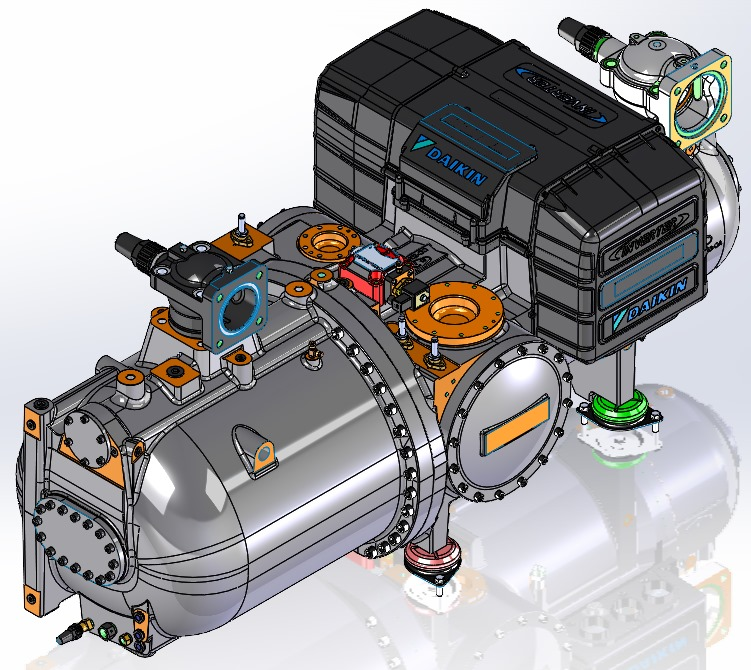
\includegraphics[width=0.6\textwidth]{img/daikin/35-A-CO1005.jpeg}
                \caption{Compressore 35-A-CO1005}
            \end{figure}
        \end{column}
    \end{columns}

    \vspace{0.2cm}
    \begin{alertblock}{Scelta Progettuale}
        Dimensionamento sovrastimato a \textbf{1000 kg} (robot + payload) per scalabilità futura e margine di sicurezza.
    \end{alertblock}
\end{frame}
% Slide 2: Requisiti Veicolo
\begin{frame}
    \frametitle{Requisiti Veicolo}
    \begin{alertblock}{Requisiti Veicolo}
        \begin{itemize}
            \item \textbf{Capacità Carico}: 1000 kg.
            \item \textbf{Velocità Max}: 1 m/s (sicurezza).
            \item \textbf{Autonomia}: 4 ore operative.
            \item \textbf{Ambiente}: Indoor/Outdoor (asfalto, cemento).
            \item \textbf{Manovrabilità}: Omnidirezionale (parcheggio parallelo).
            \item \textbf{Economico}: Costo contenuto per dimostratore tecnologico.
        \end{itemize}
    \end{alertblock}
\end{frame}

% Slide 2: Dimensionamento Potenza
\begin{frame}
    \frametitle{Dimensionamento Potenza}
    Calcolo forza di trazione necessaria ($m=1000$ kg, $v_{max}=1$ m/s):

    \textbf{Parametri:} $\mu_r = 0.03$ (attrito volvente), $\mu_s = 0.5$ (attrito statico), $a = 0.333$ m/s$^2$
    \vspace{0.2cm}
    \begin{columns}
        \column{0.48\textwidth}
        \textbf{In Piano:}
        \begin{equation*}
            \begin{aligned}
                F_r     & = \mu_r \cdot m \cdot g = 294 \text{ N} \\
                F_a     & = m \cdot a = 333 \text{ N}             \\
                F_{tot} & = 627 \text{ N}
            \end{aligned}
        \end{equation*}
        $$P_{piano} \approx 627 \text{ W}$$

        \column{0.48\textwidth}
        \textbf{Pendenza 10\% ($\theta=5.7^\circ$):}
        \begin{equation*}
            \begin{aligned}
                F_{\parallel} & = mg\sin\theta = 974 \text{ N}       \\
                F_r           & = \mu_r mg\cos\theta = 293 \text{ N} \\
                F_a           & = 333 \text{ N}                      \\
                F_{tot}       & = 1600 \text{ N}
            \end{aligned}
        \end{equation*}
        $$P_{salita} \approx \textbf{1.6 kW}$$
    \end{columns}
\end{frame}

% Slide 3: Selezione Batteria
\begin{frame}
    \frametitle{Selezione Batteria}
    \begin{columns}
        \column{0.6\textwidth}
        \textbf{FlashBattery LiFePO4} (Litio-Ferro-Fosfato)
        \begin{itemize}
            \item \textbf{Tensione}: 51.2 V nominali (44-59.2 V).
            \item \textbf{Capacità}: 105 Ah.
            \item \textbf{Energia Totale}: 5.38 kWh.
            \item \textbf{Energia Disponibile} (80\% DOD): \textbf{4.30 kWh}.
            \item \textbf{Corrente}: 105 A continua, 210 A picco.
        \end{itemize}
        \vspace{0.1cm}
        \begin{block}{Verifica Autonomia}
            $$E_{disponibile} = 4.30 \text{ kWh} > 4 \text{ kWh (requisito)}$$
            \textbf{Margine:} 7.5\%

        \end{block}
        \column{0.4\textwidth}
        \centering
        
\includegraphics[width=0.5\textwidth]{batteria/front_view.jpeg}
    \end{columns}
\end{frame}

% Slide 4: Selezione Motori
\begin{frame}
    \frametitle{Selezione Motori: CFR MRT05}
    Configurazione: \textbf{2 Ruote Motrici Sterzanti} (Motorwheels) + 2 Caster (diagonali).

    \begin{columns}
        \column{0.42\textwidth}
        \textbf{Specifiche per ruota:}
        \begin{itemize}
            \item \textbf{Trazione}:
                  \begin{itemize}
                      \item Potenza: 500 W (S2-60min)
                      \item Coppia Nom.: 37 Nm
                      \item Coppia Picco: 180 Nm
                      \item Rapporto riduzione: 1:21
                  \end{itemize}
            \item \textbf{Sterzo}:
                  \begin{itemize}
                      \item Potenza: 300 W
                      \item Coppia: 34 Nm
                      \item Rapporto riduzione: 1:45.56
                  \end{itemize}
            \item \textbf{Encoder}: SIN/COS (FTS1)
        \end{itemize}

        \column{0.54\textwidth}
        {\small
            \begin{block}{Verifica Coppia}
                Raggio ruota: $r = 0.099$ m

                \textbf{Piano:}
                $$\tau_{tot} = F_{tot} \cdot r \approx 62 \text{ Nm}$$
                $$\tau_{ruota} = \tau_{tot}/2 \approx 31 \text{ Nm}$$
                $$\tau_{nom} = 37 \text{ Nm} \Rightarrow \textbf{Margine 18\%}$$

                \textbf{Salita 10\%:}
                $$\tau_{tot} \approx 159 \text{ Nm}$$
                $$\tau_{ruota} \approx 79.5 \text{ Nm}$$
                $$\tau_{picco} = 180 \text{ Nm} \Rightarrow \textbf{OK}$$
            \end{block}
        }
    \end{columns}
\end{frame}
\begin{frame}
    \frametitle{Selezione Motori: CFR MRT05}
    \begin{columns}
        \column{0.4\textwidth}
        \centering
        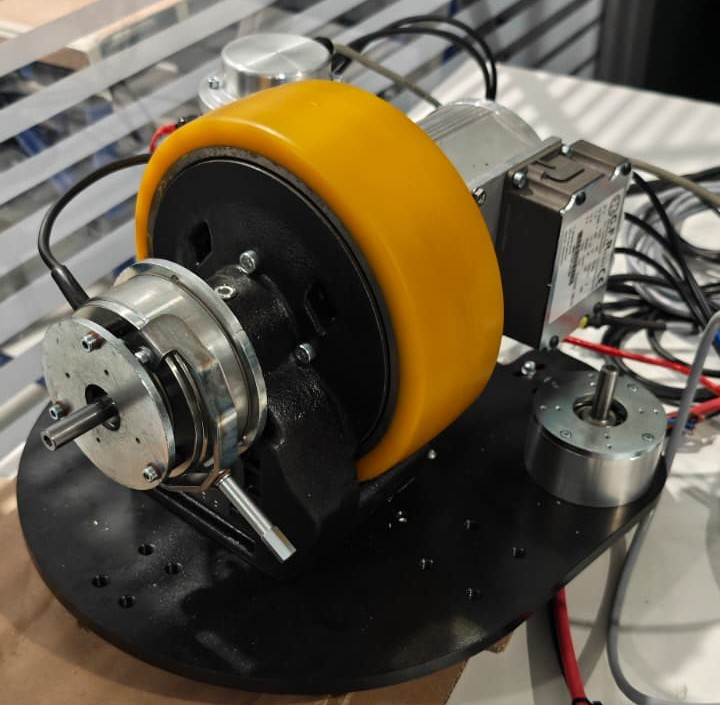
\includegraphics[width=0.8\textwidth]{img/motore/side_view_1.jpeg}
        \column{0.5\textwidth}
        \centering
        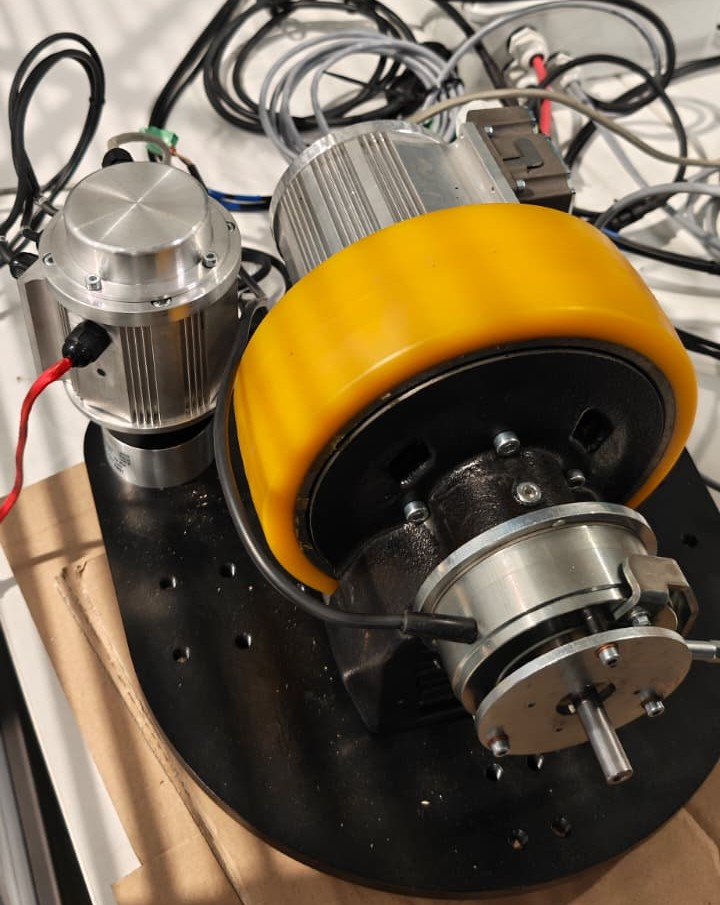
\includegraphics[width=0.6\textwidth]{img/motore/side_view_2.jpeg}
    \end{columns}

\end{frame}
% Slide 5: Architettura Hardware - Parte 1
\begin{frame}
    \frametitle{Architettura Hardware: Computazione e Sensoristica}
    \begin{itemize}
        \item \textbf{Computer di Bordo}: LattePanda Sigma
              \begin{itemize}
                  \item Intel Core i5-1340P (12 core, 16 thread)
                  \item 32GB RAM LPDDR5-6400
                  \item Ubuntu 24.04 + ROS 2 Jazzy
              \end{itemize}
        \item \textbf{LiDAR}: Livox Mid-360
              \begin{itemize}
                  \item FOV: 360° × 59° (-7° a +52°)
                  \item 200k pts/s, portata 70m
                  \item IMU 6-assi integrata (ICM40609)
              \end{itemize}
        \item \textbf{Encoder}: SIN/COS (FTS1) integrati nelle motoruote
        \item \textbf{Sonde Temperatura}: RTD (STS1) per monitoraggio termico motori
    \end{itemize}
\end{frame}

% Slide 6: Architettura Hardware - Parte 2
\begin{frame}
    \frametitle{Architettura Hardware: Alimentazione e Controllo}
    \begin{itemize}
        \item \textbf{Driver Motori}: MicroPhase Mini-Traction Power (4×)
              \begin{itemize}
                  \item Supporto CANopen CiA 402
                  \item 48V, 75A continua, 120A boost (5s)
                  \item Controllo motori PMAC
              \end{itemize}
        \item \textbf{Comunicazione}: Waveshare USB-CAN-A
              \begin{itemize}
                  \item CAN 2.0A/B, velocità fino a 1 Mbps
                  \item Resistenza terminazione 120$\Omega$ commutabile
              \end{itemize}
        \item \textbf{Convertitori DC-DC}: Meanwell
              \begin{itemize}
                  \item SD-25B-12: 48V → 12V, 25W (LiDAR)
                  \item SD-100D-12: 48V → 12V, 102W (SBC)
              \end{itemize}
        \item \textbf{Caricabatterie}: Zivan NG3
              \begin{itemize}
                  \item 48V, 60A configurabile, profilo CC-CV per LiFePO4
                  \item Comunicazione CAN con BMS, tempo ricarica: 2-3h
              \end{itemize}
    \end{itemize}
\end{frame}

% Slide 7: Foto Componenti Hardware
\begin{frame}
    \frametitle{Componenti Hardware}
    \begin{columns}
        \column{0.3\textwidth}
        \centering
        \textbf{LattePanda Sigma}

        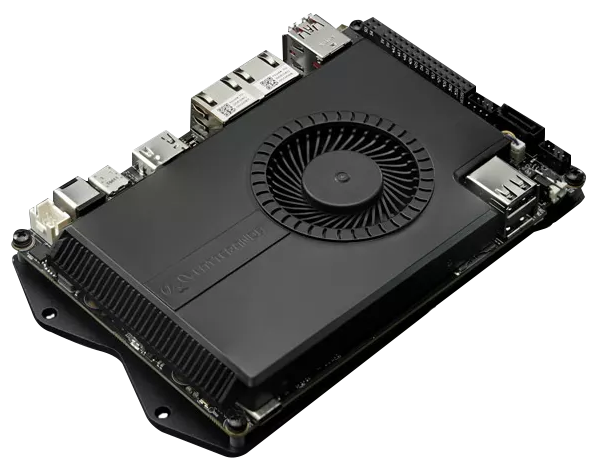
\includegraphics[width=0.7\textwidth]{img/3/lattepanda_sigma2.png}

        \vspace{0.3cm}
        \textbf{Driver Mini-Traction Power}

        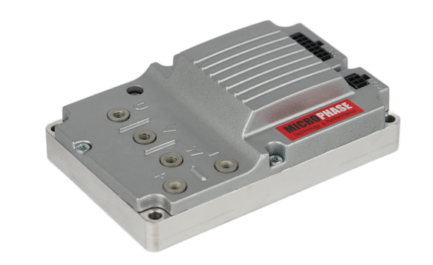
\includegraphics[width=0.7\textwidth]{img/3/mini-traction-power.png}

        \column{0.3\textwidth}
        \centering
        \textbf{Livox Mid-360}

        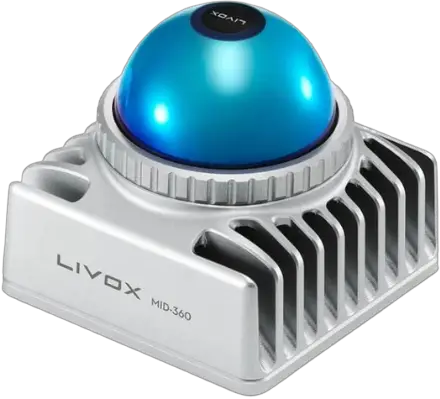
\includegraphics[width=0.6\textwidth]{img/3/livox_mid360.png}

        \vspace{0.3cm}
        \textbf{USB-CAN-A Adapter}

        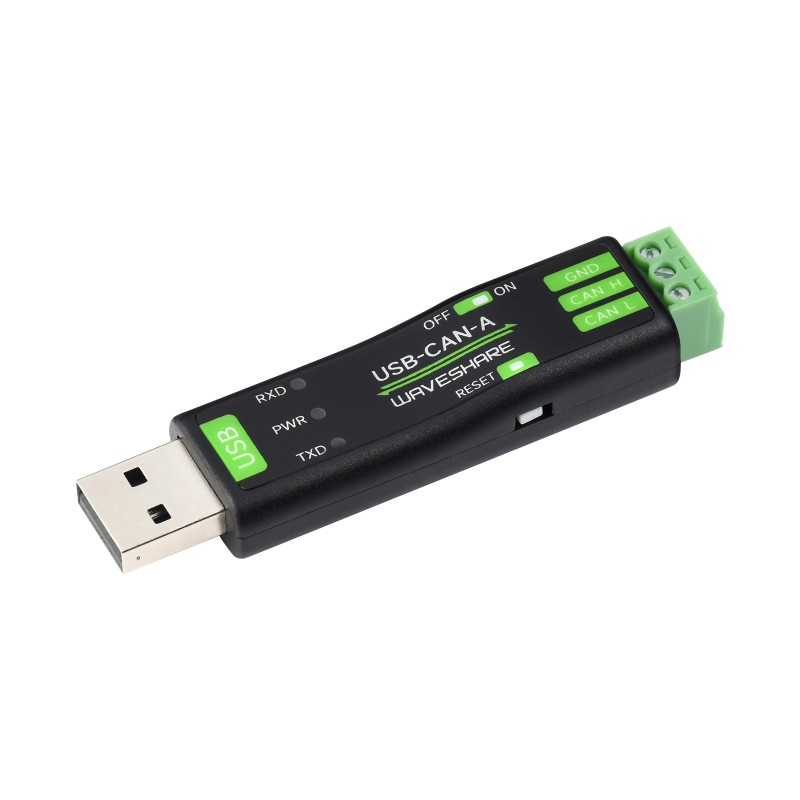
\includegraphics[width=0.6\textwidth]{img/3/usb_can_a.jpg}
    \end{columns}
\end{frame}

% Slide 7: Telaio
\begin{frame}
    \frametitle{Telaio e Struttura Meccanica}
    \begin{columns}
        \column{0.5\textwidth}
        \textbf{Caratteristiche:}
        \begin{itemize}
            \item Massa: $\sim$70 kg
            \item Profili acciaio $30 \times 30 \times 2.6$ mm
            \item Rinforzi $20 \times 20 \times 2$ mm
            \item Dimensioni: $1.8 \times 1.0$ m
            \item Piastre montaggio 5 mm
            \item Trattamento: zincatura
        \end{itemize}

        \vspace{0.3cm}
        \textbf{Progettazione:}
        \begin{itemize}
            \item CAD: SolidWorks
            \item Analisi FEM: FASTRAN
        \end{itemize}

        \column{0.5\textwidth}
        \centering
        
\includegraphics[width=\textwidth]{telaio/disegno_side.png}
    \end{columns}
\end{frame}

% Slide 8: Analisi FEM
\begin{frame}
    \frametitle{Analisi agli Elementi Finiti (FEM)}
    \textbf{Verifica strutturale} con software FASTRAN sotto carico 1000 kg.

    \vspace{0.3cm}
    \begin{columns}
        \column{0.5\textwidth}
        \centering
        \textbf{Mappa delle Deformazioni}

        
\includegraphics[width=0.8\textwidth]{telaio/fem_telaio_dettaglio_3}

        \column{0.5\textwidth}
        \centering
        \textbf{Mappa delle Deformazioni}

        
\includegraphics[width=0.9\textwidth]{telaio/fem_telaio_dettaglio_2}
    \end{columns}

    \vspace{0.3cm}
    \begin{block}{Risultati}
        Deformazioni e tensioni entro limiti di sicurezza. Zone critiche localizzate nei punti di giunzione (artefatti mesh).
    \end{block}
\end{frame}

% Slide 9: Analisi Costi
\begin{frame}
    \frametitle{Analisi dei Costi}
    \begin{table}[htbp]
        \centering
        \small
        \begin{tabular}{|l|r|}
            \hline
            \textbf{Componente}             & \textbf{Costo (€)} \\
            \hline
            Motoruote CFR MRT05 (2×)        & 5.480              \\
            Driver Mini-Traction Power (4×) & 1.640              \\
            Batteria FlashBattery           & 3.950              \\
            Caricabatterie Zivan NG3        & 355                \\
            LattePanda Sigma                & 563                \\
            Livox Mid-360                   & 659                \\
            Telaio, lamierati e caster      & 2.356              \\
            Cablaggi e messa in opera       & 1.800              \\
            Accessori (DC-DC, USB-CAN, SSD) & 429                \\
            \hline
            \textbf{Totale}                 & \textbf{17.232}    \\
            \hline
        \end{tabular}
    \end{table}

    \vspace{0.3cm}
    \begin{block}{Considerazioni}
        Costo contenuto rispetto a soluzioni commerciali (ordine di grandezza inferiore). Dimostratore tecnologico economico per validazione concetto.
    \end{block}
\end{frame}


% --- Section 4 ---
% Sezione 4: Modelli Cinematici e Controllo
\section{Modellazione Cinematica e Controllo}

\begin{frame}
    \frametitle{Modello a Biciclo Sterzante}
    \textbf{Semplificazione}: ruote sullo stesso asse $\rightarrow$ ruota virtuale unica per asse

    \vspace{0.3cm}

    \textbf{Equazioni Cinematiche}
    \begin{equation*}
        \begin{cases}
            \dot{x}      = v \cos(\theta+\beta) \\
            \dot{y}      = v \sin(\theta+\beta) \\
            \dot{\theta} = \frac{v\cos(\beta)}{l_f+l_r}\left(\tan(\delta_f)-\tan(\delta_r)\right)
        \end{cases}
    \end{equation*}

    dove:
    \begin{align*}
        v     & =  \frac{r(\omega_f \cos\delta_f + \omega_r \cos\delta_r)}{2\cos(\beta)}                                    \\
        \beta & =  \tan^{-1}\left(\frac{l_f \tan(\delta_r) + l_r \tan(\delta_f)}{l_f + l_r}\right) \quad \text{(side-slip)}
    \end{align*}

    \vspace{0.2cm}
\end{frame}
\begin{frame}
    \begin{block}{Vantaggi}
        \begin{itemize}
            \item Testato in letteratura.
            \item Modello dinamico disponibile e controllato con successo con LQR.
        \end{itemize}
    \end{block}
    \begin{alertblock}{Svantaggi: Singolarità}
        \begin{itemize}
            \item $\beta \rightarrow \infty$ se $\delta_f$ o $\delta_r \rightarrow \pi/2$ (tangente infinita)
            \item \textbf{Crab/Spin impossibile}: se $v=0$ allora $\omega_f = \omega_r = 0 \Rightarrow \dot{\theta}=0$
        \end{itemize}
    \end{alertblock}
\end{frame}

\begin{frame}
    \frametitle{Modello a Doppia Ruota Sterzante: Vincoli Non-Olonomi}
    \textbf{Vincolo di non slittamento} per ruota $i \in \{f, r\}$:

    \vspace{0.2cm}

    Velocità punto contatto ruota nel body frame:
    \begin{equation*}
        \mathbf{v}_i^b = \begin{bmatrix}
            \dot{x}_c \mp \dot{\theta}\frac{W}{2} \\
            \dot{y}_c \pm \dot{\theta}\frac{L}{2}
        \end{bmatrix}
    \end{equation*}

    \textbf{Versori}: normale $\mathbf{n}_i = \begin{bmatrix}
            -\sin(\delta_i) \\
            \cos(\delta_i)
        \end{bmatrix}$, parallelo $\mathbf{u}_i = \begin{bmatrix}
            \cos(\delta_i) \\
            \sin(\delta_i)
        \end{bmatrix}$

    \textbf{Condizione di non slittamento}: $\mathbf{n}_i^T \mathbf{v}_i^b = 0$
    \begin{equation*}
        -\sin(\delta_i)\left(\dot{x}_c \mp \dot{\theta}\frac{W}{2}\right) + \cos(\delta_i)\left(\dot{y}_c \pm \dot{\theta}\frac{L}{2}\right) = 0
    \end{equation*}

    \vspace{0.1cm}

    \textbf{Vincolo di puro rotolamento}: $\mathbf{u}_i^T \mathbf{v}_i^b = r\omega_i$
    \begin{equation*}
        \cos(\delta_i)\left(\dot{x}_c \mp \dot{\theta}\frac{W}{2}\right) + \sin(\delta_i)\left(\dot{y}_c \pm \dot{\theta}\frac{L}{2}\right) = r\omega_i
    \end{equation*}

    \vspace{0.2cm}

    \small{$(f): L/2, W/2$; $(r): -L/2, -W/2$}
\end{frame}

\begin{frame}
    \frametitle{Cinematica Diretta: Matrice dei Vincoli Estesa}
    \textbf{Sistema sovradeterminato} (4 equazioni, 3 incognite):

    \begin{equation*}
        \mathbf{A}_{ext}^T \dot{\mathbf{q}} = \mathbf{b}
    \end{equation*}

    dove:
    \begin{equation*}
        \mathbf{A}_{ext}^T = \begin{bmatrix}
            -\sin(\delta_f) & \cos(\delta_f) & \frac{W}{2}\sin(\delta_f) - \frac{L}{2}\cos(\delta_f)  \\
            -\sin(\delta_r) & \cos(\delta_r) & -\frac{W}{2}\sin(\delta_r) + \frac{L}{2}\cos(\delta_r) \\
            \cos(\delta_f)  & \sin(\delta_f) & -\frac{W}{2}\cos(\delta_f) - \frac{L}{2}\sin(\delta_f) \\
            \cos(\delta_r)  & \sin(\delta_r) & \frac{W}{2}\cos(\delta_r) - \frac{L}{2}\sin(\delta_r)
        \end{bmatrix}
        , \quad
        \mathbf{b} = \begin{bmatrix}
            0 \\ 0 \\ r\omega_f \\ r\omega_r
        \end{bmatrix}
    \end{equation*}

    \textbf{Soluzione ai minimi quadrati} (pseudoinversa di Moore-Penrose):
    \begin{equation*}
        \dot{\mathbf{q}} = \mathbf{A}_{ext}^\dagger \mathbf{b} = \left(\mathbf{A}_{ext}^T \mathbf{A}_{ext}\right)^{-1} \mathbf{A}_{ext}^T \mathbf{b}
    \end{equation*}
\end{frame}

\begin{frame}
    \frametitle{Cinematica Diretta: Forma Compatta}
    \textbf{Soluzione finale} nel body frame:

    \begin{equation*}
        \begin{bmatrix}
            \dot{x}_c \\ \dot{y}_c \\ \dot{\theta}
        \end{bmatrix}
        = \frac{r}{2}
        \begin{bmatrix}
            \cos(\delta_f) & \cos(\delta_r) \\
            \sin(\delta_f) & \sin(\delta_r) \\
            a_{13}         & a_{23}
        \end{bmatrix}
        \begin{bmatrix}
            \omega_f \\ \omega_r
        \end{bmatrix}
    \end{equation*}

    dove i coefficienti $a_{13}$, $a_{23}$ dipendono da $\delta_f$, $\delta_r$, $L$, $W$:
    \begin{align*}
        a_{13} & = \frac{2(L\sin(\delta_f) - W\cos(\delta_f))}{L^2 + W^2} \\
        a_{23} & = \frac{2(W\cos(\delta_r) - L\sin(\delta_r))}{L^2 + W^2}
    \end{align*}
\end{frame}
\begin{frame}
    \begin{block}{Vantaggi}
        \begin{itemize}
            \item Trasformabile facilmente in frame globale e viceversa (pre-mnoltiplicando $R(\theta)$/$R^T(\theta)$)
            \item \textbf{Nessuna singolarità cinematica} per qualsiasi $\delta_f, \delta_r$ (Pseudoinversa mai singolare)
            \item Gestisce \textbf{crab} ($\dot{x}_c=0$, $\dot{y}_c\neq0$) e \textbf{spin} ($\dot{x}_c=\dot{y}_c=0$, $\dot{\theta}\neq0$)
        \end{itemize}
    \end{block}
    \begin{alertblock}{Svantaggi}
        \begin{itemize}
            \item No modellazione dinamica (forze, inerzie)
            \item No modellazione ruote libere
            \item Soluzione ai minimi quadrati: possibilità di rompere vincoli non-olonomi
        \end{itemize}
    \end{alertblock}
\end{frame}

\begin{frame}
    \frametitle{Centro Istantaneo di Rotazione (ICR)}
    \textbf{Concetto}: punto attorno al quale il veicolo sta ruotando in un dato istante

    \vspace{0.3cm}

    L'ICR si trova all'\textbf{intersezione degli assi di rotazione delle ruote} (perpendicolari alla direzione di avanzamento):

    \begin{equation}
        \begin{bmatrix}
            x_{ICR} \\ y_{ICR}
        \end{bmatrix}
        = \mathbf{p}_i^b + s_i \begin{bmatrix}
            -\sin(\delta_i) \\ \cos(\delta_i)
        \end{bmatrix}
        \quad i \in \{f, r\}
    \end{equation}

    \textbf{Distanza da ICR}: $R_i = |s_i|$ (raggio di curvatura per ruota $i$)

    \vspace{0.2cm}

    \textbf{Condizione di compatibilità} (moto senza slittamento):
    \begin{equation}
        \dot{\theta} R_i = r\omega_i \quad \Rightarrow \quad R_r \omega_f = R_f \omega_r
    \end{equation}

    \small{Caso $\delta_f \parallel \delta_r$: ICR $\to \infty$, traslazione pura con $\omega_f = \omega_r$}
\end{frame}

\begin{frame}
    \frametitle{Cinematica Inversa: Modello a Biciclo}
    \textbf{Problema}: dato $(\dot{x}_d, \dot{y}_d, \dot{\theta}_d)$, calcolare $(\delta_f, \delta_r, \omega_f, \omega_r)$

    \vspace{0.3cm}

    \textbf{Passo 1}: Calcolare velocità e side-slip desiderati
    \begin{align}
        v_d     & = \sqrt{\dot{x}_d^2 + \dot{y}_d^2} \nonumber       \\
        \beta_d & = \atanyx{\dot{y}_d}{\dot{x}_d} - \theta \nonumber
    \end{align}

    \textbf{Passo 2}: Risolvere sistema per angoli di sterzo (definendo $S = \tan(\beta_d)$, $D = \frac{l\dot{\theta}_d}{v_d \cos(\beta_d)}$)
    \begin{align}
        \delta_f & = \arctan\left(S + \frac{l_f}{l} D\right) \\
        \delta_r & = \arctan\left(S - \frac{l_r}{l} D\right)
    \end{align}

    \textbf{Passo 3}: Calcolare $\omega_f$, $\omega_r$ da raggi ICR $R_f$, $R_r$ e condizione compatibilità
\end{frame}

\begin{frame}
    \frametitle{Cinematica Inversa Biciclo: Caso $\dot{\theta}_d = 0$ (Parte 1)}
    \textbf{Derivazione per traslazione pura}

    \vspace{0.3cm}

    Quando $\dot{\theta}_d = 0$, l'ICR $\to \infty$ e le direzioni di avanzamento delle ruote diventano parallele.

    \vspace{0.3cm}

    \textbf{Step 1}: Imporre $\delta_f = \delta_r = \delta$ (sterzi paralleli)

    \vspace{0.3cm}

    \textbf{Step 2}: Dalla relazione del side-slip angle:
    \begin{equation}
        \beta_d = \tan^{-1}\left(\frac{l_f + l_r}{l_f + l_r}\tan(\delta)\right) = \delta
    \end{equation}

    \vspace{0.3cm}

    Quindi il side-slip angle coincide con l'angolo di sterzo quando le ruote sono parallele.
\end{frame}

\begin{frame}
    \frametitle{Cinematica Inversa Biciclo: Caso $\dot{\theta}_d = 0$ (Parte 2)}
    \textbf{Calcolo angoli di sterzo e velocità}

    \vspace{0.3cm}

    \textbf{Step 3}: Combinando $\beta_d = \delta$ con $\beta_d = \atanyx{\dot{y}_d}{\dot{x}_d} - \theta$:
    \begin{equation}
        \delta_f = \delta_r = \delta = \atanyx{\dot{y}_d}{\dot{x}_d} - \theta
    \end{equation}

    \vspace{0.3cm}

    \textbf{Step 4}: Le velocità angolari sono uguali (condizione di compatibilità per ICR $\to \infty$):
    \begin{equation}
        \omega_f = \omega_r = \frac{v_d}{r} = \frac{\sqrt{\dot{x}_d^2 + \dot{y}_d^2}}{r}
    \end{equation}
\end{frame}

\begin{frame}
    \frametitle{Cinematica Inversa: Modello Bisteer}
    \textbf{Soluzione diretta dai vincoli di non-slittamento}:

    \vspace{0.3cm}

    \textbf{Angoli di sterzo} (dalle eq. non-slip):
    \begin{align}
        \delta_f & = \atanyx{\dot{y}_d + \dot{\theta}_d \frac{L}{2}}{\dot{x}_d - \dot{\theta}_d \frac{W}{2}} \\
        \delta_r & = \atanyx{\dot{y}_d - \dot{\theta}_d \frac{L}{2}}{\dot{x}_d + \dot{\theta}_d \frac{W}{2}}
    \end{align}

    \textbf{Velocità angolari ruote} (dalle eq. rotolamento):
    \begin{align}
        \omega_f & = \frac{(\dot{y}_d + \dot{\theta}_d \frac{L}{2}) \sin(\delta_f) + (\dot{x}_d - \dot{\theta}_d \frac{W}{2}) \cos(\delta_f)}{r} \\
        \omega_r & = \frac{(\dot{y}_d - \dot{\theta}_d \frac{L}{2}) \sin(\delta_r) + (\dot{x}_d + \dot{\theta}_d \frac{W}{2}) \cos(\delta_r)}{r}
    \end{align}

    \textbf{Caso speciale $\dot{\theta}_d = 0$}: $\delta_f = \delta_r = \atanyx{\dot{y}_d}{\dot{x}_d}$, $\omega_f = \omega_r = \frac{v_d}{r}$
\end{frame}

\begin{frame}
    \frametitle{Setup Simulazioni}
    \textbf{Parametri Robot e Attuatori}
    \begin{itemize}
        \item Dimensioni: $L = 2$ m, $W = 1$ m, $r = 0.198$ m
        \item Dinamica attuatori: modello 1$^\circ$ ordine $P(s) = \frac{K}{\tau s + 1}$
              \begin{itemize}
                  \item Trazione: $K_{\omega} = 1$, $\tau_\omega = 1$ s, $\omega_{max} = 10$ rad/s
                  \item Sterzo: $K_{\delta} = 1$, $\tau_\delta = 2$ s, $\delta_{max} = \pm 120^\circ$
              \end{itemize}
    \end{itemize}

    \vspace{0.3cm}

    \textbf{Traiettorie di Test}
    \begin{enumerate}
        \item \textbf{Straight}: linea retta verso Est ($v_{ref} = 0.5$ m/s, $T = 5$ s)
        \item \textbf{Arc}: arco circolare ($R = 3$ m, $v_{ref} = 0.6$ m/s, $\omega = 0.2$ rad/s, $T = 8$ s)
        \item \textbf{Crab}: traslazione laterale Nord ($v_{ref} = 0.4$ m/s, $T = 5$ s)
        \item \textbf{Spin}: rotazione sul posto ($\omega_{ref} = \pi/6$ rad/s, $T = 6$ s)
    \end{enumerate}

    \vspace{0.2cm}
    \small{Metrica: RMSE posizione e orientamento vs. traiettoria desiderata}
\end{frame}

\begin{frame}
    \frametitle{Schema di Controllo: Feedforward (Catena Aperta)}
    \begin{figure}
        \centering
        
\includegraphics[width=0.95\textwidth]{4/FF_scheme.pdf}
    \end{figure}

    \textbf{Caratteristiche}:
    \begin{itemize}
        \item Nessun feedback dallo stato misurato
        \item Cinematica inversa calcola input da traiettoria desiderata
        \item Dinamica attuatori introduce ritardi non compensati
        \item Errori si accumulano senza correzione
    \end{itemize}
\end{frame}

\begin{frame}
    \frametitle{Risultati Feedforward: Traiettoria Arc}
    \begin{figure}
        \centering
        
\includegraphics[width=0.85\textwidth]{4/curved_east_to_north_feedforward_bicycle.png}
        \caption{Modello Bicycle - Traiettoria circolare (Feedforward)}
    \end{figure}
\end{frame}

\begin{frame}
    \frametitle{Risultati Feedforward: Traiettoria Arc}
    \begin{figure}
        \centering
        
\includegraphics[width=0.85\textwidth]{4/curved_east_to_north_feedforward_bisteer.png}
        \caption{Modello Bisteer - Traiettoria circolare (Feedforward)}
    \end{figure}
\end{frame}

\begin{frame}
    \frametitle{Risultati Feedforward: Confronto e Analisi}
    \begin{columns}
        \column{0.5\textwidth}
        \begin{table}
            \centering
            \tiny
            \begin{tabular}{@{}lcccc@{}}
                \toprule
                \textbf{Traiett.} & \textbf{Mod.} & \textbf{Supp.} & \textbf{Pos. [mm]}                & \textbf{Orient. [$^\circ$]}      \\
                \midrule
                \multirow{2}{*}{Str.}
                                  & Bic.          & x              & 418.05                            & 0.00                             \\
                                  & Bis.          & x              & 418.05                            & 0.00                             \\
                \midrule
                \multirow{2}{*}{Arc}
                                  & Bic.          & x              & 749.92                            & 20.80                            \\
                                  & Bis.          & x              & \textbf{694.70}                   & \textbf{18.85}                   \\
                \midrule
                \multirow{2}{*}{Cra.}
                                  & Bic.          & --             & \textcolor{red}{\textbf{1154.82}} & 0.00                             \\
                                  & Bis.          & x              & \textbf{334.44}                   & 0.00                             \\
                \midrule
                \multirow{2}{*}{Spi.}
                                  & Bic.          & --             & 0.00                              & \textcolor{red}{\textbf{103.93}} \\
                                  & Bis.          & x              & 0.00                              & \textbf{25.93}                   \\
                \bottomrule
            \end{tabular}
        \end{table}

        \column{0.45\textwidth}
        \textbf{Osservazioni}:
        \begin{itemize}
            \item Bicycle FALLISCE su Crab e Spin (singolarità)
            \item Bisteer gestisce tutte le manovre
            \item Errori elevati per assenza feedback
        \end{itemize}
    \end{columns}
\end{frame}

\begin{frame}
    \frametitle{Schema di Controllo: PID + Feedforward}
    \begin{figure}
        \centering
        
\includegraphics[width=\textwidth]{4/FF_PID.pdf}
    \end{figure}
\end{frame}
\begin{frame}
    \frametitle{Dettagli Implementazione PID}
    \textbf{Legge di controllo}:
    \begin{align}
        e^b           & = R^T(\theta) \begin{bmatrix} x_d - x \\ y_d - y \\ \theta_d - \theta \end{bmatrix} \quad \text{(errore in body frame)} \nonumber \\
        u_i(t)        & = K_{p,i} e_i^b + K_{i,i} \int e_i^b \, dt + K_{d,i} \frac{d e_i^b}{dt}, \quad i \in \{x,y,\theta\} \nonumber                     \\
        \dot{q}_{cmd} & = \dot{q}_d + u \quad \text{(velocità corrette in global frame)} \nonumber
    \end{align}
\end{frame}

\begin{frame}
    \frametitle{Dettagli Implementazione PID}
    \textbf{Guadagni utilizzati}:
    \begin{table}
        \centering
        \small
        \begin{tabular}{cccccc}
            \toprule
            \textbf{Comp.} & $K_p$ & $K_i$ & $K_d$ & $I_{max}$ & $N$ \\
            \midrule
            $x, y$         & 0.3   & 0.05  & 0.1   & 2         & 20  \\
            $\theta$       & 0.2   & 0.02  & 0.05  & 1         & 20  \\
            \bottomrule
        \end{tabular}
    \end{table}

    \vspace{0.3cm}

    \textbf{Accorgimenti implementativi}:
    \begin{itemize}
        \item \textbf{Derivata filtrata}: $D(s) = \frac{K_d s}{s/N + 1}$ (riduce rumore)
        \item \textbf{Anti-windup}: saturazione integrale per evitare wind-up
        \item \textbf{Scaling proporzionale}: mantiene rapporto tra $u_x, u_y$ sotto $v_{max}$
        \item \textbf{Saturazione angolare}: $|u_\theta| \leq \omega_{max}$
    \end{itemize}
\end{frame}

\begin{frame}
    \frametitle{Risultati PID+FF: Traiettoria Arc}
    \begin{figure}
        \centering
        
\includegraphics[width=0.85\textwidth]{4/curved_east_to_north_pid_bicycle.png}
        \caption{Modello Bicycle - Traiettoria circolare (PID+FF)}
    \end{figure}
\end{frame}

\begin{frame}
    \frametitle{Risultati PID+FF: Traiettoria Arc}
    \begin{figure}
        \centering
        
\includegraphics[width=0.85\textwidth]{4/curved_east_to_north_pid_bisteer.png}
        \caption{Modello Bisteer - Traiettoria circolare (PID+FF)}
    \end{figure}
\end{frame}

\begin{frame}
    \frametitle{Risultati PID+FF: Confronto e Miglioramenti}
    \begin{columns}
        \column{0.55\textwidth}
        \begin{table}
            \centering
            \tiny
            \begin{tabular}{@{}lcccc@{}}
                \toprule
                \textbf{Traiett.} & \textbf{Mod.} & \textbf{Supp.} & \textbf{Pos. [mm]}                & \textbf{Orient. [$^\circ$]}      \\
                \midrule
                \multirow{2}{*}{Str.}
                                  & Bic.          & x              & 233.96                            & 0.00                             \\
                                  & Bis.          & x              & 233.96                            & 0.00                             \\
                \midrule
                \multirow{2}{*}{Arc}
                                  & Bic.          & x              & 231.27                            & 12.53                            \\
                                  & Bis.          & x              & \textbf{229.57}                   & \textbf{11.66}                   \\
                \midrule
                \multirow{2}{*}{Cra.}
                                  & Bic.          & --             & \textcolor{red}{\textbf{1154.82}} & 0.00                             \\
                                  & Bis.          & x              & \textbf{187.17}                   & 0.00                             \\
                \midrule
                \multirow{2}{*}{Spi.}
                                  & Bic.          & --             & 0.00                              & \textcolor{red}{\textbf{103.93}} \\
                                  & Bis.          & x              & 0.00                              & \textbf{16.14}                   \\
                \bottomrule
            \end{tabular}
        \end{table}

        \column{0.45\textwidth}
        \textbf{Miglioramenti vs FF}:
        \begin{itemize}
            \item Str: $418 \to 234$ mm ($-44\%$)
            \item Arc: $695 \to 230$ mm ($-67\%$)
            \item Crab: $334 \to 187$ mm ($-44\%$)
            \item Spin: $26^\circ \to 16^\circ$ ($-38\%$)
        \end{itemize}
    \end{columns}
\end{frame}

\begin{frame}
    \frametitle{Conclusioni: Confronto Modelli Cinematici}
    \begin{columns}
        \column{0.5\textwidth}
        \textbf{Modello Biciclo}
        \begin{itemize}
            \item[+] Testato in letteratura
            \item[+] Estensione dinamica disponibile
            \item[-] \textbf{Singolarità}: Crab e Spin impossibili
            \item[-] $\beta \to \infty$ per $\delta \to \pi/2$
        \end{itemize}

        \column{0.5\textwidth}
        \textbf{Modello Bisteer}
        \begin{itemize}
            \item[+] \textbf{Nessuna singolarità}
            \item[+] Supporta tutte le manovre
            \item[+] Prestazioni migliori con PID
            \item[!] Pseudoinversa può violare vincoli
        \end{itemize}
    \end{columns}

    \vspace{0.5cm}

    \textbf{Scelta finale}: \textcolor{green!60!black}{\textbf{Modello Bisteer}} per maggiore versatilità e robustezza
\end{frame}


% --- Section 5 ---
\section{Architettura Software e Comunicazione}

% --- Section 6 ---
% Sezione 6: Sviluppi Futuri
\section{Conclusioni e Sviluppi Futuri}

\begin{frame}
    \frametitle{Risultati Raggiunti}
    \begin{block}{Progettazione Completa AMR}
        \begin{itemize}
            \item Requisiti: 1000 kg capacità, 1 m/s, 4h autonomia, €15k budget
            \item Configurazione 2 motorwheels + 2 caster (diagonali)
            \item Componenti: CFR MRT05, FlashBattery LiFePO4, Livox Mid-360, LattePanda Sigma
            \item Verifiche energetiche: motori 18\% margine piano, batteria 7.5\% margine
        \end{itemize}
    \end{block}

    \begin{block}{Modellazione e Controllo}
        \begin{itemize}
            \item Modello Bicycle: singolarità su crab/spin (FAIL)
            \item Modello Bisteer: vincoli non-olonomi, least-squares, nessuna singolarità
            \item Simulazioni: RMSE < 1.5 cm su 4 traiettorie (straight, arc, crab, spin)
            \item PID+Feedforward: riduzione RMSE ~30\%, settling time < 2s
        \end{itemize}
    \end{block}

    \begin{block}{Integrazione Tecnologie}
        \begin{itemize}
            \item FAST-LIO 2 (iEKF + ikd-Tree) per SLAM > 100 Hz
            \item CANopen CiA 402 per controllo deterministic motori (PDO, heartbeat)
        \end{itemize}
    \end{block}
\end{frame}

\begin{frame}
    \frametitle{Sviluppi Futuri}
    \begin{enumerate}
        \item \textbf{Implementazione Software}
              \begin{itemize}
                  \item Integrazione ROS 2 per architettura modulare
                  \item Deployment algoritmo FAST-LIO 2 su LattePanda Sigma
                  \item Interfaccia CANopen per controllo motori in tempo reale
              \end{itemize}

        \item \textbf{Validazione Sperimentale}
              \begin{itemize}
                  \item Test su campo presso stabilimento Daikin Ariccia
                  \item Misurazione prestazioni: precisione tracking, autonomia, affidabilità
                  \item Ottimizzazione parametri controllo su dati reali
              \end{itemize}

        \item \textbf{Estensioni}
              \begin{itemize}
                  \item Fleet management per coordinamento multi-robot
                  \item Integrazione con MES aziendale per pianificazione trasporti
                  \item Sensori addizionali: telecamere RGB-D, safety laser scanner
              \end{itemize}
    \end{enumerate}
\end{frame}
\begin{frame}
    \frametitle{Conclusioni e Sviluppi Futuri}
    \begin{columns}
        \column{0.5\textwidth}
        \begin{block}{Stato Attuale}
            \begin{itemize}
                \item Definizione requisiti e componenti completata.
                \item Analisi cinematica e scelta algoritmi (FAST-LIO 2) effettuata.
                \item Acquisizione hardware in corso.
            \end{itemize}
        \end{block}

        \column{0.5\textwidth}
        \begin{block}{Prossimi Passi}
            \begin{enumerate}
                \item \textbf{Assemblaggio}: Costruzione telaio e cablaggio elettrico.
                \item \textbf{Integrazione Software}: Setup ROS 2 e driver CANopen.
                \item \textbf{Test in Campo}:
                \begin{itemize}
                    \item Mapping dello stabilimento di Ariccia.
                    \item Test di navigazione con ostacoli dinamici.
                \end{itemize}
                \item \textbf{Integrazione WMS}: Interfacciamento con gestionale di magazzino.
            \end{enumerate}
        \end{block}
    \end{columns}
\end{frame}


\end{document}